%%%%%%%%%%%%%%%%%%%%%%%%%%%%%%%%%%%%%%%%%%%%%%%%%%%%%%%%
%%%%%%%%%%%%%%%%% START 1_ARTICLE.tex %%%%%%%%%%%%%%%%%%
%%%%%%%%%%%%%%%%%%%%%%%%%%%%%%%%%%%%%%%%%%%%%%%%%%%%%%%%
    \begin{adjmulticols}{2}{0mm}{0mm}
%\chapter{Introduction}
\lettrine[lines=2]{\bfseries\color{black}K}{nowledge. Evidence. Truth.} Qualitative researchers often refrain from using such grandiose terms (in fact, some of us even have problems writing these words without using ironic capitalization or metaphysical scare quotes), because they seem tainted by a metaphysical realism in which social reality is ‘out there’, waiting to be empirically studied and causally explained by the objective methods of social science (Denzin, Lincoln \& Giardina, 2006). In other words, these extravagant terms convey the idea of social science as a neutral purveyor of objective facts about the world, the so-called correspondence theory of truth. Opposing this idea, qualitative researchers have long insisted that social scientific knowledge is socially, culturally, historically and politically embedded (Gergen, 1973). This rhetorical strategy, however, raises an important question: if qualitative researchers embrace a philosophy of flux and abandon the idea of social scientific truths as mirrors of nature (Rorty, 1979), what kind of truth do we hope to provide to our readers? In other words, what is the point of reading qualitative research? Taking inspiration from Paul Ricoeur’s (1970) distinction between a hermeneutics of suspicion%
    \pagenote{ Ricoeur’s now-famous phrase ‘hermeneutics of suspicion’ is actually nowhere to be found in \textit{Freud and Philosophy} (1970), but came up at a later date (Scott-Baumann, 2009).}
and a hermeneutics of faith, this article sketches out two possible answers: a critical approach and a phenomenological approach. The article first examines the \textit{critical approach}, which exposes hidden truths to educate and emancipate its readers. In the past few years, however, this approach has come under scrutiny. Eve Sedgwick (2003), for instance, has forcefully rejected what she calls paranoid reading; Bruno Latour (2004b) has provocatively argued that critique has ‘run out of steam’, and Rita Felski (2015) has cogently identified the limits of critique. Summarizing these arguments, we can say that the critical approach has been faulted for its tautological reasoning, its reductionist analytical strategies and its arrogant approach to other people. The article then goes on to explore the \textit{phenomenological approach}, which points out unnoticed truths to reverberate and resonate with its readers. It is argued that this self-consciously ‘weak’ approach helps us circumvent the issues associated with the critical approach. In the interests of full disclosure, I should state that I consider my own research to belong to this latter camp, so this special issue constitutes a welcome opportunity to explore the phenomenon of resonance: what is it? When does it occur? And what does it do? To enhance readability, I here provide a schematic preview of the differences between the critical approach and the phenomenological approach (see \tref{tab:p4:1}):
    \end{adjmulticols}
\FloatBarrier
\noindent
\begin{table}[htb]
\centering % centering kan tilføjes her (optional)
\caption{} % caption indstillinger er under preamble/macros
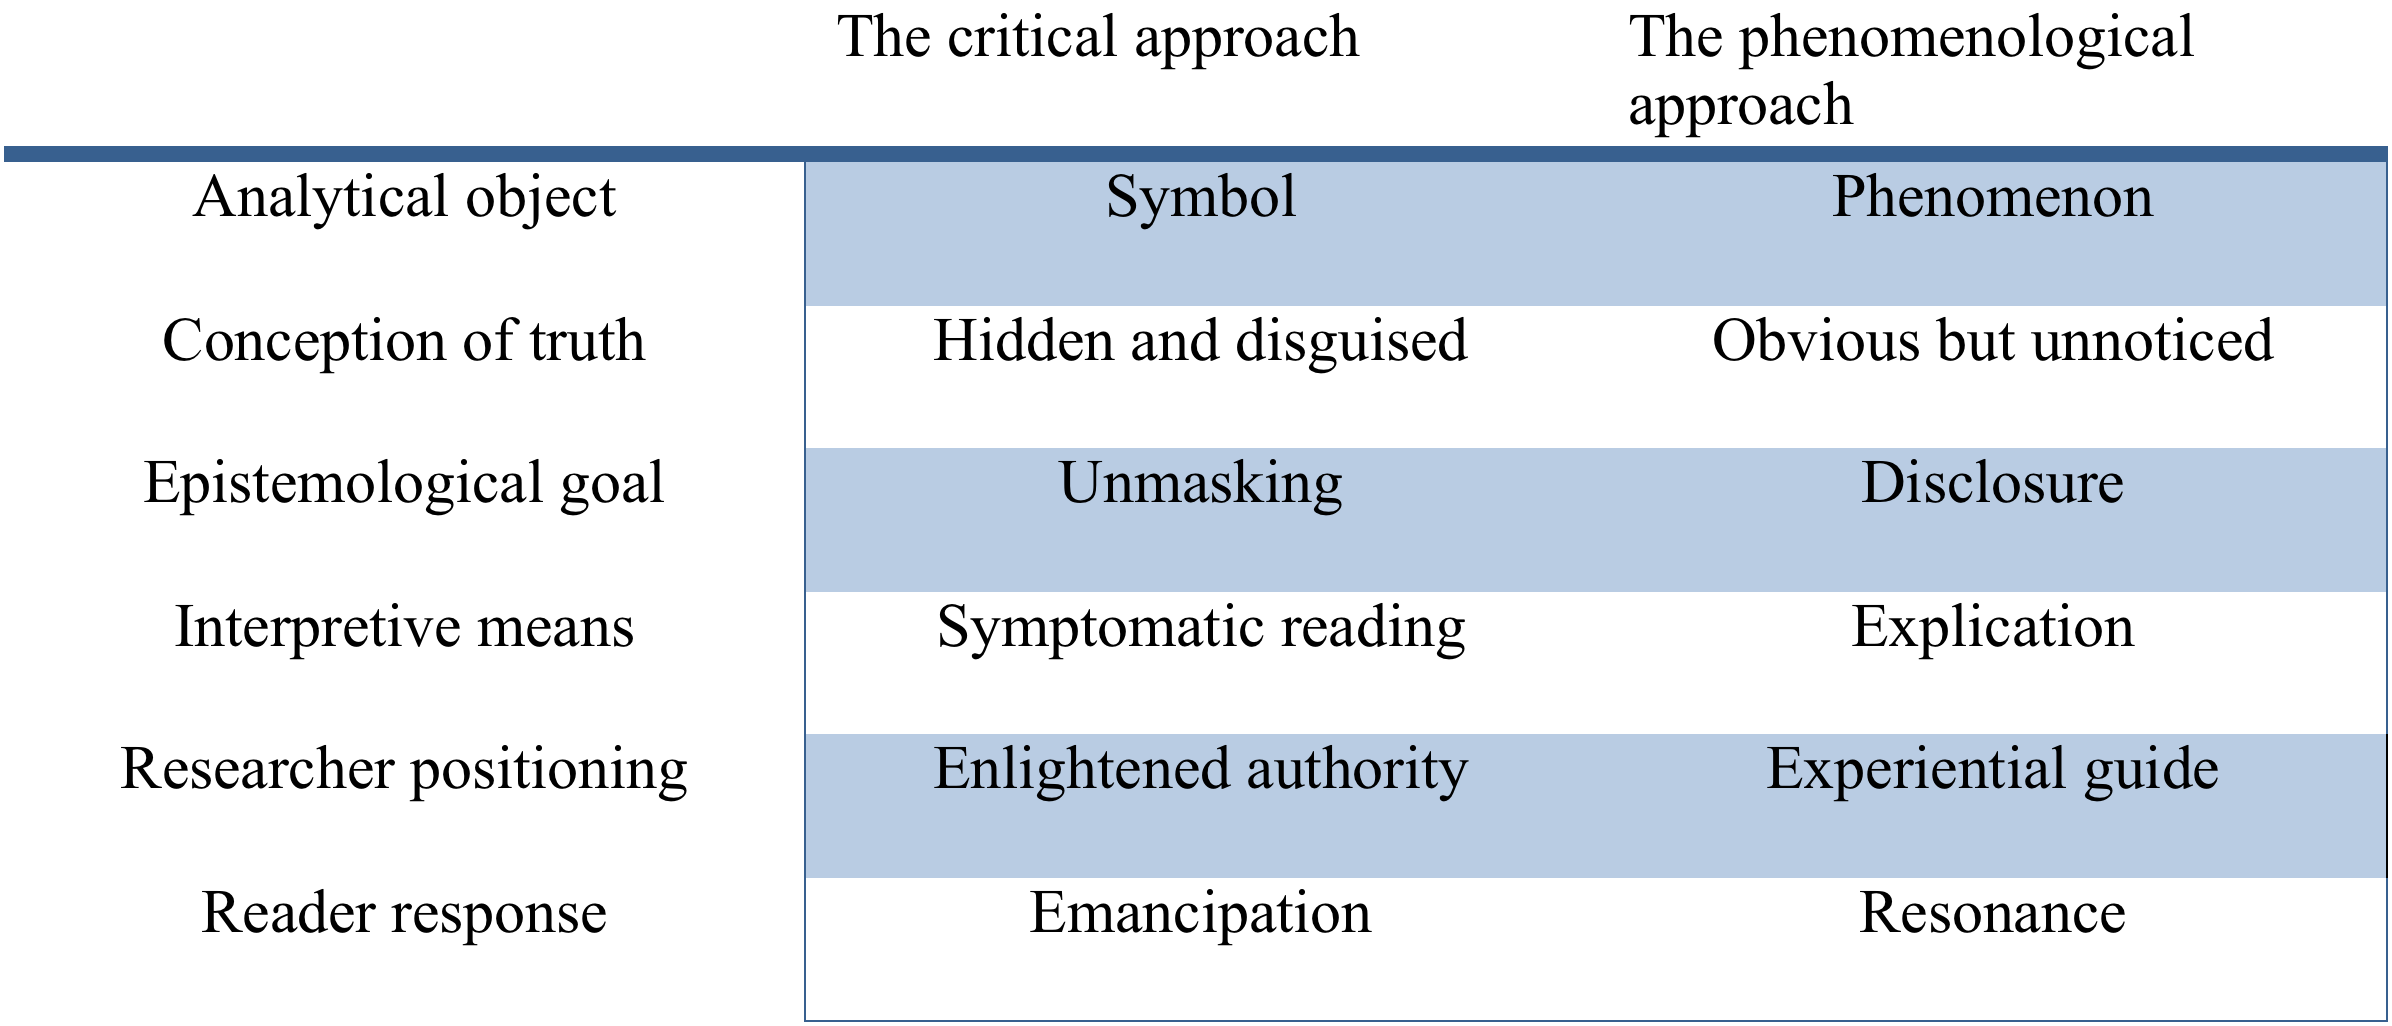
\includegraphics[width=0.9\linewidth]{paper4/p4_data/p4-fig1.png}
\label{tab:p4:1}
\end{table}
\FloatBarrier
    \begin{adjmulticols}{2}{0mm}{0mm}
\chapter{The Critical Approach: A Hermeneutics of Suspicion}
What since Ricoeur (1970) has become known as the hermeneutics of suspicion is a collection of interpretive strategies that relies on an architecture of meaning layered in terms of surface/depth, manifest/latent or apparent/hidden, with a deep gulf separating these two layers. As Marx (1971) famously declared: ‘All science would be superfluous if the outward appearance and the essence of things directly coincided’ (p. 817). Accordingly, while the hermeneutics of suspicion views the social world as inherently meaningful, it treats all surface meanings with suspicion, because such outward appearances are presumed to conceal a deeper and truer layer of meaning. For Marx, this hidden truth was class struggle; for Freud, it was libidinous drives; for Nietzsche, it was the will to power. Although operating beneath the surface, these structures are taken to regulate people’s behaviour and condition their experiences. Ricoeur’s masters of suspicion therefore shared a profound mistrust of people’s ordinary everyday experiences, which they primarily approached in terms of false consciousness. As a result, the critical approach does not take its analytical object (whether this be a statement, a dream or a common household item) at face value, but treats it as a symbol in which ‘a direct, primary, literal meaning designates, in addition, another meaning which is indirect, secondary, and figurative and which can be apprehended only through the first’ (Ricoeur, 1974: 12f). In other words, the hermeneutics of suspicion uses its analytical object as a gateway to a deeper level of meaning. Freud, for instance, saw the manifest content of a dream as little more than a carrier for the significant content, which is latent. As Frieden (1990) explains: ‘Freud’s dream theories rely on the basic opposition between manifest and latent dream contents, between actual dream images and concealed meaning, explicit and implicit layers, surface and depth structures’ (p. 21).

To unlock its secrets, critical interpreters read the analytical object in accordance with a theoretical apparatus such as psychoanalysis or Marxism. Using this theoretical master key, the critical interpreter performs a symptomatic reading of the object, which plumbs its depths and digs out ‘a latent meaning behind a manifest one’ (Jameson, 2013: 45). The hermeneutics of suspicion thus involves an element of esotericism in that it presupposes the specific style of reading that is necessary for \textit{that} particular form of decoding (Josselson, 2004). The purpose of a symptomatic reading is to penetrate the surface of the analytical object, get in touch with its underlying layer of meaning and unmask this repressed truth. Such demystification eschews the object’s apparent meaning in order to uncover the truth that lurks beneath its surface. As Ricoeur (1970) argues, ‘This hermeneutics is not an explication of the object, but a tearing off of masks, an interpretation that reduces disguises’ (p. 30). The quest for such hidden truth presupposes some sort of explanatory structure that lies beneath and explains the surface appearances (e.g. class struggle, libidinous drives, will to power). While a recourse to such grand metanarratives has lost some momentum in our postmodern times, Felski (2015) convincingly argues that many strands of poststructuralism can still be characterized as suspicious, since they retain the basic architecture of meaning while simply inverting the relationship between surface and depth: ‘It is superficiality that is now the hidden truth, while interiority is demoted to a deceptive façade’ (p. 80). While suspicious scholars traditionally ‘dig down’ to excavate a hidden layer, and poststructuralists ‘stand back’ to denaturalize the analytical object, both approaches require the interpreter to tear away a veil of appearances in order to expose what is \textit{really} going on to the reader. In both forms of interpretation, the researcher is thus positioned as an enlightened authority that has already discovered some truth and must now lead others to see it, too.

Since this truth transcends everyday experience, it is not important that lay people and other outsiders immediately understand or agree to it. In fact, a cardinal objective of the hermeneutics of suspicion is to debunk ordinary people’s beliefs and educate them on the hidden forces that drive their existence. This is thought to emancipate them from the thrall of false consciousness. ‘It is the lesson of Spinoza’, Ricoeur (1970) argues, ‘one first finds himself a slave, he understands his slavery, he rediscovers himself free within understood necessity’ (p. 35). The truth shall set you free. Truth in the critical approach can thus be understood as a movement from secrecy to exposure, from ignorance to knowledge, or from darkness to light. This kind of learning can be considered as a formation of critical consciousness, the ability to see through deceptive appearances, or simply as the ‘unlearning of bullshit’ (Colaizzi, 1978). Brinkmann (2012) calls this critical strategy ‘making the hidden obvious’ and uses Ian Parker’s (1996) analysis of the directions on the back of a tube of children’s toothpaste as an example (p. 188f): 
    \blockquote{\textnormal{\scshape\underline{Directions for Use}}
    \\Choose a children’s brush that has a small head and add a pea-sized amount of \enquote{Punch \& Judy}--toothpaste. To teach your child to clean teeth, stand behind and place your hand under the child’s chin to tilt head back and see mouth. Brush both sides of teeth as well as tops. Brush after breakfast and last thing at night. Supervise the brushing of your child’s teeth until the age of eight. If your child is taking fluoride treatment, seek professional advice concerning daily intake.
    \\Contains 0.8 per cent Sodium Monofluorophosphate.}
To the untrained eye, these directions may at first glance \textit{look like} innocuous instructions for caring for one’s child, but Parker argues that they \textit{actually} contain a rich tapestry of power, violence and domination. According to Parker’s analysis, ‘Punch initiates the infant and the audience (of children) into a form of violent (ir)rationality, a surplus of enjoyment in the puppet narrative which is also, for the battered baby, and Judy, beyond the pleasure principle’ (p. 191f). This symptomatic reading unmasks the exercise of power that lurks behind an otherwise innocuous everyday object. As a result, the toothpaste text can no longer be read with an innocent eye. 

\section{Distrusting The Hermeneutics of Suspicion}
For many years, the merits of the critical approach seemed self-evident as social science prided itself on exposing hidden power structures. Additionally, the very notion of ‘critique’ is normatively powerful: after all, who wants to be associated with the uncritical, the gullible and the naïve? Gayatri Spivak (1996), however, has argued that ‘Deconstruction, if one wants a formula, is, among other things, a persistent critique of what one cannot not want’ (p. 28). In that spirit, the concept of critique has recently come under scrutiny in academic fields like queer theory, sociology and literary studies: Eve Sedgwick (2003), for instance, has forcefully rejected what she calls paranoid reading; Bruno Latour (2004b) has provocatively argued that critique has ‘run out of steam’, and Rita Felski (2015) has cogently identified the limits of critique. Two things need mentioning with regard to this burgeoning field of so-called ‘postcritique’ (Anker \& Felski, 2017). First, while a backlash against critique may sound like nostalgic yearning for natural scientific realism, these postcritical scholars are emphatically \textit{not} seeking to replace meanings and interpretations with objectivity and brute facts. Paraphrasing Susan Sontag (1990), they readily accept interpretation in the broad sense in which ‘there are no facts, only interpretations’, but protest the narrower sense in which critical interpreters say, ‘Look, don’t you see that X is really—or, really means—A?’. Secondly, any critique of critique can logically be faulted for having critical aims itself, for having a blind spot regarding its own hermeneutics of suspicion (Barnwell, 2016). Postcritical scholars are well aware of this performative paradox. Felski (2015), for instance, explicitly avoids lapsing into a metasuspicion that exposes, subverts and dismisses critique. Her book is not ‘against’ disagreement, objection or negative judgment. ‘I have engaged in all these activities in the preceding pages’, as she states in its conclusion (p. 187). The goal of postcritique is not to do away with critique, but to treat it simply as one language game among others, to challenge the fact that critique has become ‘a mandatory injunction rather than a possibility among possibilities’ (Sedgwick, 2003: 125). 

Apart from its hegemonic status, however, what seems to be the matter with critique? According to postcritical scholars, there are at least three additional problems. The first issue is the strongly tautological nature of critique. According to Sedgwick (2003), its fierce aversion to surprise means that critical interpretation requires bad news to be known in advance. Presuming the inescapability of some harmful entity X, however, leads researchers to circularity: it is first argued that no area of inquiry is immune to the influence of X, because X is an omnipresent systemic condition that colours everything that we say and do. This assumption leads to an ‘anticipatory mimetic strategy’, in which the influence of X is presumed so as not to catch us off guard. In the end, this interpretation ends up proving its own assumption, namely that X is significant. We inevitably end up at the predetermined destination, but, as Felski (2008) asks, ‘what virtue remains in the act of unmasking when we know full well what lies beneath the mask?’ (p. 1). This circular reasoning leads us to a second flaw of critical interpretation, namely that it is (or at least can be) peculiarly reductionist. The critical approach treats its analytical objects as symbols that, when properly read, yield hidden truths about large-scale, \enquote{hypostasized villains} (Fleissner, 2017) like Neoliberalism, Patriarchy, Technocracy or Capitalism. The analytical object thereby serves as a reflection, expression, or manifestation of one of these larger entities. The problem with this interpretive strategy is not that it is necessarily wrong (in fact, it might be alarmingly accurate), but that the analytical object is reduced to allegory and ceases to matter. As Latour (2005) argues: ‘If some “social factor” is transported through intermediaries, then everything important is in the factor, not in the intermediaries. For all practical purposes, it can be substituted by them without any loss of the nuances’ (p. 105). The critical approach strips the analytical object of agency and reduces it to a neutral instrument that simply transports meaning from one domain to another.

Finally, there is the arrogant demeanour of critique. According to Latour (2004b), critical scholars have always known better than ordinary actors, often dismissing and deconstructing these people’s naïve beliefs. ‘You have to learn to become suspicious of everything people say because of course we all know that they live in the thralls of a complete \textit{illusio} of their real motives’ (p. 229). Critical interpreters are presumed to have privileged access to the world compared to ordinary actors, whose understandings are taken to spring from hidden entities of which they remain blissfully unaware. Accordingly, critique adopts a rather condescending stance towards other people, who are treated as self-deluded pawns: ‘Forgive them Father, for they know not what they do’ (Latour, 1996: 199). When language is taken to speak through people, for instance, individuals become unwitting mouthpieces for certain discourses, and we can safely brush away their own understandings of what they say and do. This critical strategy can also be found outside the walls of academia. Not too long ago here in Denmark, for instance, a male Member of Parliament suggested that female left-wing politicians who oppose increased immigration control are acting under the sway of repressed sexual desire for Middle Eastern men.%
    \pagenote{ Incredible as it may sound, this accusation actually happened. Here is a link to the published letter (in Danish): \url{http://www.fyens.dk/debat/Socialdemokrater-svigter-kvinderne/artikel/3130263}.} 
\par
Conversely, politicians who favour increased immigration control are often accused of acting out of latent racism rather than legitimate political concerns. In both cases, the assumption is not only that the other party is mistaken about their own motives (‘Look, don’t you see that what you’re doing, X, is really—or, really means—A?’), but also that, if they only realized the truth of this interpretation, they would presumably change their wicked ways. Just like that, political \textit{disagreement} turns into epistemological \textit{deficiency}. In the words of Ricoeur (1981): ‘Ideology is the thought of my adversary, the thought of the other. He does not know it, but I do’ (p. 186). Summarizing these arguments, we can say that the critical approach has been faulted for its tautological reasoning, its reductionist analytical strategies and its arrogant approach to other people.

\chapter{The Phenomenological Approach: A Hermeneutics of Everydayness}
How do we overcome the shortcomings of the critical approach? There are almost as many suggestions as there are detractors. In this section, however, I want to sketch out a phenomenological approach derived from Division I of Martin Heidegger’s magnum opus \textit{Being and Time} (1927/2008). According to Hubert Dreyfus’s (1991) highly influential interpretation of this book, this first division relies on a hermeneutics of everydayness (equivalent to Ricoeur’s hermeneutics of faith), while the second division goes on to apply a hermeneutics of suspicion. ‘The job of Division I is thus to call attention to those aspects of everyday activity that that activity itself makes it difficult for us to notice’ (p. 36). Calling attention to unnoticed aspects of everyday activity is in fact a succinct characterization of the phenomenological approach that follows. The overarching principle of Heidegger’s – and, indeed, any—phenomenological approach is captured in the famous maxim ‘To the things themselves!’ (\textit{Zu den Sachen selbst!}) (Carman, 2006). But what exactly are such things? According to Heidegger, they are neither physical objects nor brute matters of fact, but \textit{phenomena} defined as ‘that which shows itself in itself’ (p. 51). Importantly, such phenomena cannot be reduced to mere appearances, and Heidegger ferociously opposed any such metaphysical distinctions between appearance and reality: ‘Behind the phenomena of phenomenology’, he argued, ‘there is essentially nothing else’ (p. 60). Phenomenology thus relies on a flat architecture of meaning: human being is interpretation ‘all the way down’ (Dreyfus, 1991). There is nothing lurking \textit{behind} our everyday practices that can be invoked to explain them; there is only interpretation \textit{within} these practices, and the researcher’s job is to ‘interpret the interpretation embodied in our current practices in as comprehensive and responsible a way as possible’ (Dreyfus, 1980: 14). 
But if phenomenological inquiry is concerned with ‘that which shows itself in itself’, then what is the point of doing it? What does it let us see that we do not already know? ‘Manifestly, it is something that first and foremost precisely does \textit{not} show itself’, Heidegger argued, ‘something that, in contrast to what first and foremost shows itself, is hidden, but is at the same time something that essentially belongs to that which first and foremost shows itself, and belongs to it in such a way as to constitute its meaning and ground’ (p. 59). The first law of phenomenology states that what is closest to us in our everyday activity remains furthest from us in terms of our ability to take it up and understand it (Thomson, 2009). As Wittgenstein (2009) said: ‘The aspects of things that are most important for us are hidden because of their simplicity and familiarity. (One is unable to notice something—because it is always before one's eyes.)’ (§129). The purpose of phenomenology is to point out these obvious but unnoticed aspects. This process is known as disclosure, Heidegger’s translation of the Greek word \textit{aletheia}, which means to discover or draw out of concealment—to make the unnoticed noticed. In this process, the phenomenological researcher acts as an experiential guide who uses meticulous attention to detail and evocative examples to convey their analysis. The phenomenologist’s job is to point out details and make them ‘light up’ in order to get the reader to notice them. The phenomenologist’s endeavour is thus somewhat similar to Toril Moi’s (2017) description of Sherlock Holmes’s investigative process: ‘It’s not that the others look at the surface, whereas Sherlock looks beneath it. It is that he pays attention to details they didn’t think to look at’ (p. 186). In other words, the phenomenological researcher applies the hermeneutical conception of interpretation as explication (\textit{Auslegung}), which means to lay out, unfold and elucidate (Dreyfus, 1980). Such explication is related to what Albert Borgmann (1984) calls deictic discourse: ‘The word “deictic” comes from Greek \textit{deiknýnai}, which means to show, to point out, to bring to light, to set before one, and then also to explain and to teach. Speakers of deictic discourse never finally warrant the validity of what they tell but point away from themselves to what finally matters; they speak essentially as witnesses’ (p. 178). 

To achieve disclosure, phenomenological inquiry takes departure in human experience in its average everydayness. Contrary to the hermeneutics of suspicion, the hermeneutics of everydayness has faith in people’s experiences of the world. This is not to say that people always know with certainty why they are acting (phenomenology is not seeking a return to the self-transparent Cartesian subject), but that it is imperative to trace meaning back to people’s lived experiences. As Felski (2015) puts it, ‘I strive to remain on the same plane as my object of study rather than casting around for a hidden puppeteer who is pulling the strings’ (p. 6). Phenomenology thus offers understanding from within: truth may be unnoticed, undiscovered, or hidden in plain sight, but it is \textit{there}. The devil is in the details. In my own research on digital technology, I subscribe to an actor-network-inspired variant of phenomenology called postphenomenology (Aagaard, 2017). While the topic of technology will not be further explored here, I find it instructive to follow postphenomenology’s refusal to treat its analytical objects (i.e. technologies) as mere epiphenomena. Instead, postphenomenology follows Latour’s (2005) injunction to treat things as concrete and ‘worthy’ actors in their own right. The analytical object has to be treated as a fully fledged and irreducible phenomenon that is investigated in its specificity. As Don Ihde (1998) maintains: ‘The postmodern hermeneutics of things must find ways to give voices to things, to let them speak for themselves’ (p. 158). This insistence on letting things speak impedes large-scale critiques of Capitalism, Technocracy or Neoliberalism, because, at this level of abstraction, technologies are often reduced to mute symbols of such nebulous entities (Aagaard, 2017). 

\chapter{Resonance: The Phenomenological Nod of Recognition}
But if phenomenology neither discovers objective facts nor unmasks hidden truths, then what does it do? According to Max van Manen (1990), a good phenomenological description \textit{resonates} with life and evokes the phenomenological nod of recognition\textit{.} The concept of resonance derives from the words \textit{re} (back, again) and \textit{sonare} (to sound) and means to echo, reverberate, or ‘re-sound’. The goal of phenomenology is thus not to shock or surprise, but to strike a chord of familiarity with its readers. When a text resonates with the reader, it excites, stimulates and sets the person in motion. It moves the reader. What van Manen calls the ‘phenomenological nod’ is the embodied expression of such experiential resonance. As Michaele Ferguson (2009) argues, applying resonance as a validity criterion helps us steer between the tricky extremes of false universalism (‘everybody shares the same experiences’) and idiosyncratic subjectivism (‘each person’s experiences are unique’): ‘We can only generalize from these experiences for those with whom they resonate’ (p. 54). A phenomenological interpretation offers itself to anyone reading the article, but does not lay claim to universality. One of phenomenological research’s ardent critics, John Paley (2017), raises a critical objection to using resonance as a validity criterion, namely that, if the phenomenological nod is the litmus test of good research, then phenomenology cannot tell us anything that we did not already know: ‘In which case, what’s the point of it?’ (p. 71). So, is phenomenology just trite, predictable and uninformative? Not at all. By pointing toward something that has remained unnoticed and overlooked, but which we immediately recognize when it is pointed out, phenomenological research helps us notice and spell out certain important aspects of our everyday practices. 

Brinkmann (2012) calls this phenomenological strategy ‘making the obvious obvious’ and uses Iris Marion Young’s seminal article \textit{Throwing Like a Girl} (1980) as an example. In this article, Young describes how women are socialized to comport their bodies in inhibited ways when throwing (but also when walking, lifting, and so forth): while boys step forward, rotate their hips and shoulders, and hurl the ball forward, girls do not bring their whole bodies into motion. ‘Rather, the girls tend to remain relatively immobile except for their arms, and even the arm is not extended as far as it could be’ (p. 142). Girls, in other words, throw only with their forearm and elbow joint. In accordance with the criterion of resonance, Young notes that this analysis is not necessarily applicable to \textit{all }women and may also apply to some men (there is a famous picture of then President Barack Obama ‘throwing like a girl’ as he throws the ceremonial first pitch at the Washington Nationals’ 2010 home opener). Nevertheless, Young’s analysis (sadly) resonates with many of us. As Bonnie Mann (2009) puts it: ‘“Like a girl” is one of those phrases we wish didn’t make sense, and hope one day will not’ (p. 84). Young does not simply describe the overt physical movements involved in feminine body comportment, however, but meticulously analyses the meaning of such comportment: inhibited intentionality. This meaning does not lie hidden behind, beneath or beyond the phenomenon, but originates from the steady repetition of restricted movements over time. The issue is not spatial, but chronological. Young’s article certainly is not uncritical, but alters the usual direction of attack: instead of finding patriarchy hidden \textit{behind} everyday practices, Young demonstrates how it is constituted \textit{within} them. Patriarchy is not so much expressed in baseball as it is performed or enacted within it.

It should be mentioned that the phenomenological approach described here is more akin to a broad, qualitative stance than a substantial theoretical allegiance. Accordingly, the concept of resonance is in no way limited to texts that self-identify as phenomenological. In fact, the first time I remember having the phenomenological nod of recognition evoked was not at all while reading phenomenology, but when, as an undergraduate, I read Erving Goffman’s descriptions of behaviour in public places. Goffman’s knack for dissecting the micro-dramas of everyday life has led Pierre Bourdieu (1983) to characterize him as a ‘discoverer of the infinitely small’ and Howard Becker (2003) to describe his work accordingly: ‘To begin with, many of the things he gives names to are well known to us, his readers. We recognize them immediately; they are familiar experiences we have had or events we have witnessed. But, and this is a very important but, we don’t have names for these experiences and events […] We feel that we have always known it but, until Goffman gave it to us, did not know its name’ (p. 663). As an example of this uncanny ability, here is a brief excerpt from Goffman’s (1963) descriptions of civil inattention: ‘Where the courtesy is performed between two persons passing on the street, civil inattention may take the special form of eyeing the other up to approximately eight feet, during which time sides of the street are apportioned by gesture, and then casting the eyes down as the other passes – a kind of dimming of lights’ (p. 84). Reading this passage, I immediately recognized the phenomenon Goffman describes and thought to myself, ‘How have I never noticed that before?’. It’s not that my previous way of perceiving the world was somehow false or mistaken; I simply had not noticed that particular aspect of life before and was now struck by it. Accordingly, resonance does not so much penetrate a veil of ignorance as sharpen the reader’s sensory apparatus. As Latour (2004a) puts it: ‘The more you learn, the more differences exist’ (p. 213). And after reading Goffman’s texts, one’s world becomes slightly more articulated.

\chapter{Conclusion}
The critical and phenomenological approaches share a number of family resemblances. They both view mainstream psychology as flawed in its objectivism and instead take departure in an inherently meaningful social world (i.e. they are both hermeneutic). As a result, both approaches take an interpretive approach to studying human beings. Although quite similar in that respect, however, the two approaches are far from identical, and it was this article’s contention that the phenomenological approach helps us circumvent the problems that postcritical scholars have pinpointed.

First, there is the tautological notion of already knowing what you are going to find. The phenomenological approach tries to avoid this circular disposition by remaining modest, attentive and inquisitive concerning its analytical objects. Using Sedgwick’s distinction between weak and strong theory, we might say that the phenomenological approach has deliberately fashioned itself as a ‘weak’ theory that strives to give credence to the things themselves. Does this lead us back to the naïve realism that we so desperately want to avoid? To an indiscriminate acceptance of the myth of the given? This is certainly an understandable concern, since some phenomenological scholars claim that phenomenology liberates us from theory and allows us to see the light of lived experience (see Aagaard, 2017). Phenomenology, however, is emphatically \textit{not} a neutral lens through which we perceive a pre-given phenomenon, but an intellectual tool that shapes our research process all the way down to data collection: it influences what we see, which questions we ask, and what ultimately stands forth as significant (Aagaard, 2017). A weak theory, in other words, is not the same as an empty theory. This clarification clears the way for an important distinction: although phenomenology dictates what to look at (i.e. experience), it remains open as to what we may find. By mediating the research process without determining its outcome, it thereby helps us break out of the tautological loop.

Secondly, there is the issue of reductionist analytical strategies. The critical approach treats the analytical as a symbol that has to be deciphered by an enlightened authority. This manoeuvre often leads us back to the usual suspects of Discourse, Power and Capitalism. The phenomenological approach, however, does not grant much explanatory power to these macroscale entities, but treats its analytical objects as fully fledged and irreducible phenomena. We have to beware of one seemingly obvious consequence of this analytical move: to grant the idea that phenomenology is well suited for exploring phenomena at the individual level, but struggles to account for larger political and socio-economic structures. This kind of concession plays right into the stereotypical characterization of phenomenology as naïve and subjectivist (for an excellent discussion of this long-standing critique, see Greiffenhagen \& Sharrock, 2008). But phenomenology does not advocate political complicity and quietism, nor does it endorse the status quo or hinder critique, as we have seen with Young’s (1980) article. On the contrary, to give an account of political structures \textit{without} attention to how we live them is to risk an abstract objectivism that cannot grasp the lived experience of structural injustice (Mann, 2009).

Finally, there is the idea that critical scholars possess an acute awareness of the hidden structures that prefigure and mould \textit{other} people’s experiences. In the situated perspective of phenomenology, there is no external vantage point from which the researcher can assume this privileged position vis-à-vis their analytical object. On the contrary, phenomenology wants to lead us back to the everyday world, and in this endeavour it considers people’s lived experience as a helpful ally against overly restrictive understandings: when sufficiently probed, lived experience exhibits nuances that cannot be contained by crass philosophical binaries. Although it was not this article’s intention to let critique serve as a dialectical foil to phenomenology (things are not always simply as they appear, and critique certainly has its rightful place in qualitative research), this last issue constitutes a challenge to critique: when critical interpreters challenge or contradict the sentiments expressed by ordinary people, they owe us an account of the privileged position from which they make that call.
    \end{adjmulticols}